\styledchapter[Proof of concept]{oplossing}
Om de PoC daadwerkelijk te maken moet er eerst gedefinieerd worden wat de scope is en hoe de PoC eruit gaat zien. De scope brengt in beeld wat er gedaan moet worden en wat de \acrfull{mvp} is. Op de \acrshort{mvp} kan de mock up gebaseerd worden. In dit hoofdstuk wordt de scope bepaald, delen van de mock up doorgelopen, uitleg gegeven over de PoC en kwaliteit van de code. Het hoofdstuk wordt afgesloten met een conclusie en advies

\section{User requirements verzamelen}\label{sec:ch7-user-requirements-verzamelen}
Om te begrijpen wat er gebouwd moet worden kunnen de behoeftes opgeschreven worden in de vorm van user stories. Een user story is de behoefte opgeschreven in een specifieke formaat om belangrijke informatie te achterhalen \cite{agile-user-story-template}. Een bekende formaat is de \textit{Connextra template} van Mike Cohn \cite{agile-user-story-template}: "\textbf{As a [role], I can [capability], so that [receive benefit]}". De template zorgt ervoor dat de rol (role), functie (capability) en reden (benefit) bekend is. In \autoref{fig:ch7-requirements} zijn alle user stories opgesteld, gegroepeerd in Epics. Bij elke user story is ook aangegeven of het \acrshort{mvp} is, welk prioriteit het heeft en de t-shirt size. De t-shirt size is een manier om op een hoog niveau aan te geven hoeveel werk een user story vereist. Een \textbf{S} vereist weinig werk terwijl \textbf{XL} veel werk vereist.

\begin{figure}[hbt!]
  \centering
  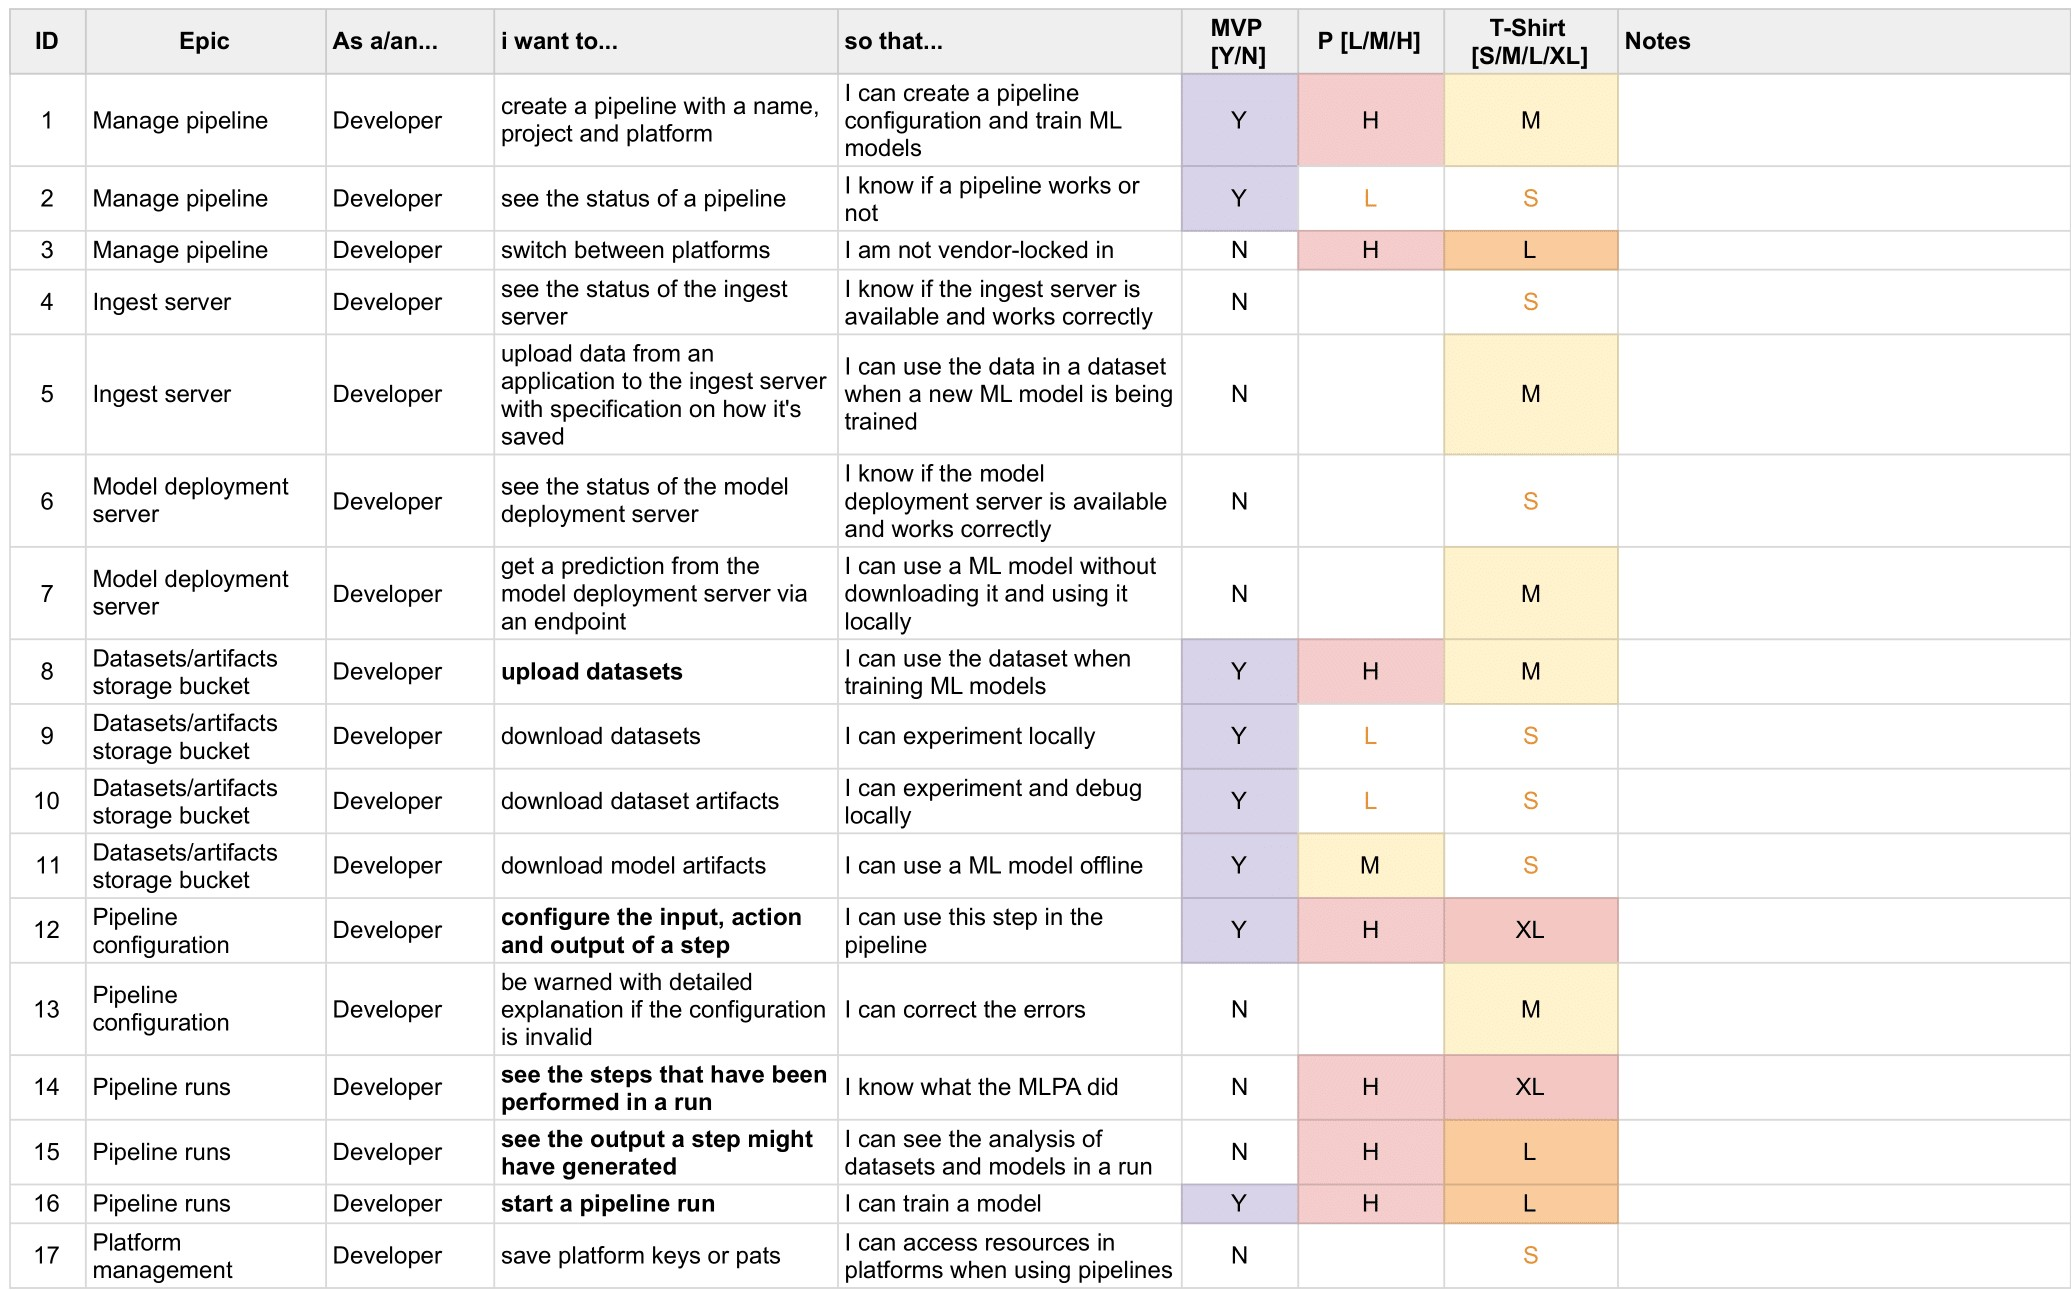
\includegraphics[width=0.99\textwidth]{chapter-7/requirements.jpg}
  \caption{Requirements opgesteld voor de proof of concept.}
  \label{fig:ch7-requirements}
\end{figure}

De user stories zijn opgesteld in samenwerking met de begeleiders van NGTI over het hele afstudeerproces. Nu de requirements zijn opgesteld, kan een Kanban bord opgericht worden om sprints te maken.

\newpage

\subsection{Requirements vertalen naar een Kanban board}\label{subsec:ch7-requirements-vertalen-naar-een-kanban-board}

\section{Mock up van de proof of concept}\label{sec:ch7-mock-up-van-de-proof-of-concept}

\section{Voorbereiding van de proof of concept}\label{sec:ch7-voorbereiding-van-de-proof-of-concept}

\subsection{Aanmaken van pipelines}\label{subsec:ch7-aanmaken-van-pipelines}
\subsection{Datasets uploaden}\label{subsec:ch7-datasets-uploaden}
\subsection{Configuratie definiëren}\label{subsec:ch7-configuratie-definieren}
\subsection{Pipeline starten}\label{subsec:ch7-pipeline-starten}
\subsection{Model downloaden}\label{subsec:ch7-model-downloaden}

% ---

\section{Conclusie}\label{sec:ch7-conclusie}
\section{Advies}\label{sec:ch7-advies}